\documentclass[a4paper,11pt]{report}
\usepackage{chuan_math_gkt}
\usetikzlibrary{angles,quotes,intersections,patterns,decorations.pathreplacing}
\chuanexamsetup

\begin{document}
\examfontsize

\examsecret{绝密$\bigstar$启用前}

\examtitle{2022年普通高等学校招生全国统一考试（全国乙卷理科）}{数\quad 学}

\noticetitle
\begin{examnotice}
\item 答卷前，考生务必将自己的姓名、准考证号填写在答题卡上. 
\item 回答选择题时，选出每小题的答案后，用铅笔把答题卡上对应题目的答案标号涂黑. 如需改动，用橡皮擦干净后，再选涂其他答案标号. 回答非选择题时，将答案写在答题卡上. 写在本试卷上无效. 
\item 考试结束后，将本试卷和答题卡一并交回. 
\end{examnotice}

\examsection{一、选择题：本题共12小题，每小题5分，共60分. 在每小题给出的四个选项中，只有一项是符合题目要求的. }
\begin{examquestions}
\item 设全集 $U=\{1,2,3,4,5\}$，集合 $M$ 满足 $\complement_U M=\{1,3\}$，则
\fourchoices{$2\in M$}{$3\in M$}{$4\notin M$}{$5\notin M$}
\item 已知 $z=1-2\mathrm{i}$，且 $z+a\overline z+b=0$，其中 $a,b$ 为实数，则
\fourchoices{$a=1,b=-2$}{$a=-1,b=2$}{$a=1,b=2$}{$a=-1,b=-2$}
\item 已知向量 $\vec a,\vec b$ 满足 $|\vec a|=1,|\vec b|=\sqrt3,|\vec a-2\vec b|=3$，则 $\vec a\cdot\vec b=$
\fourchoices{$-2$}{$-1$}{$1$}{$2$}
\item 嫦娥二号卫星在完成探月任务后，继续进行深空探测，成为我国第一颗环绕太阳飞行的人造行星. 为研究嫦娥二号绕日周期与地球绕日周期的比值，用到数列 $\{b_n\}$：$b_1=1+\dfrac1{\alpha_1}$，$b_2=1+\dfrac1{\alpha_1+\dfrac1{\alpha_2}}$，$b_3=1+\dfrac1{\alpha_1+\dfrac1{\alpha_2+\dfrac1{\alpha_3}}}$，$\cdots$，依此类推，其中 $\alpha_k\in\mathbb N^*(k=1,2,\cdots)$，则
\fourchoices{$b_1<b_5$}{$b_3<b_8$}{$b_6<b_2$}{$b_4<b_7$}
\item 设 $F$ 为抛物线 $C:y^2=4x$ 的焦点，点 $A$ 在 $C$ 上，点 $B(3,0)$，若 $|AF|=|BF|$，则 $|AB|=$
\fourchoices{$2$}{$2\sqrt2$}{$3$}{$3\sqrt2$}
\newpage
\item 执行下边的程序框图，输出的 $n=$
\begin{tightcenter}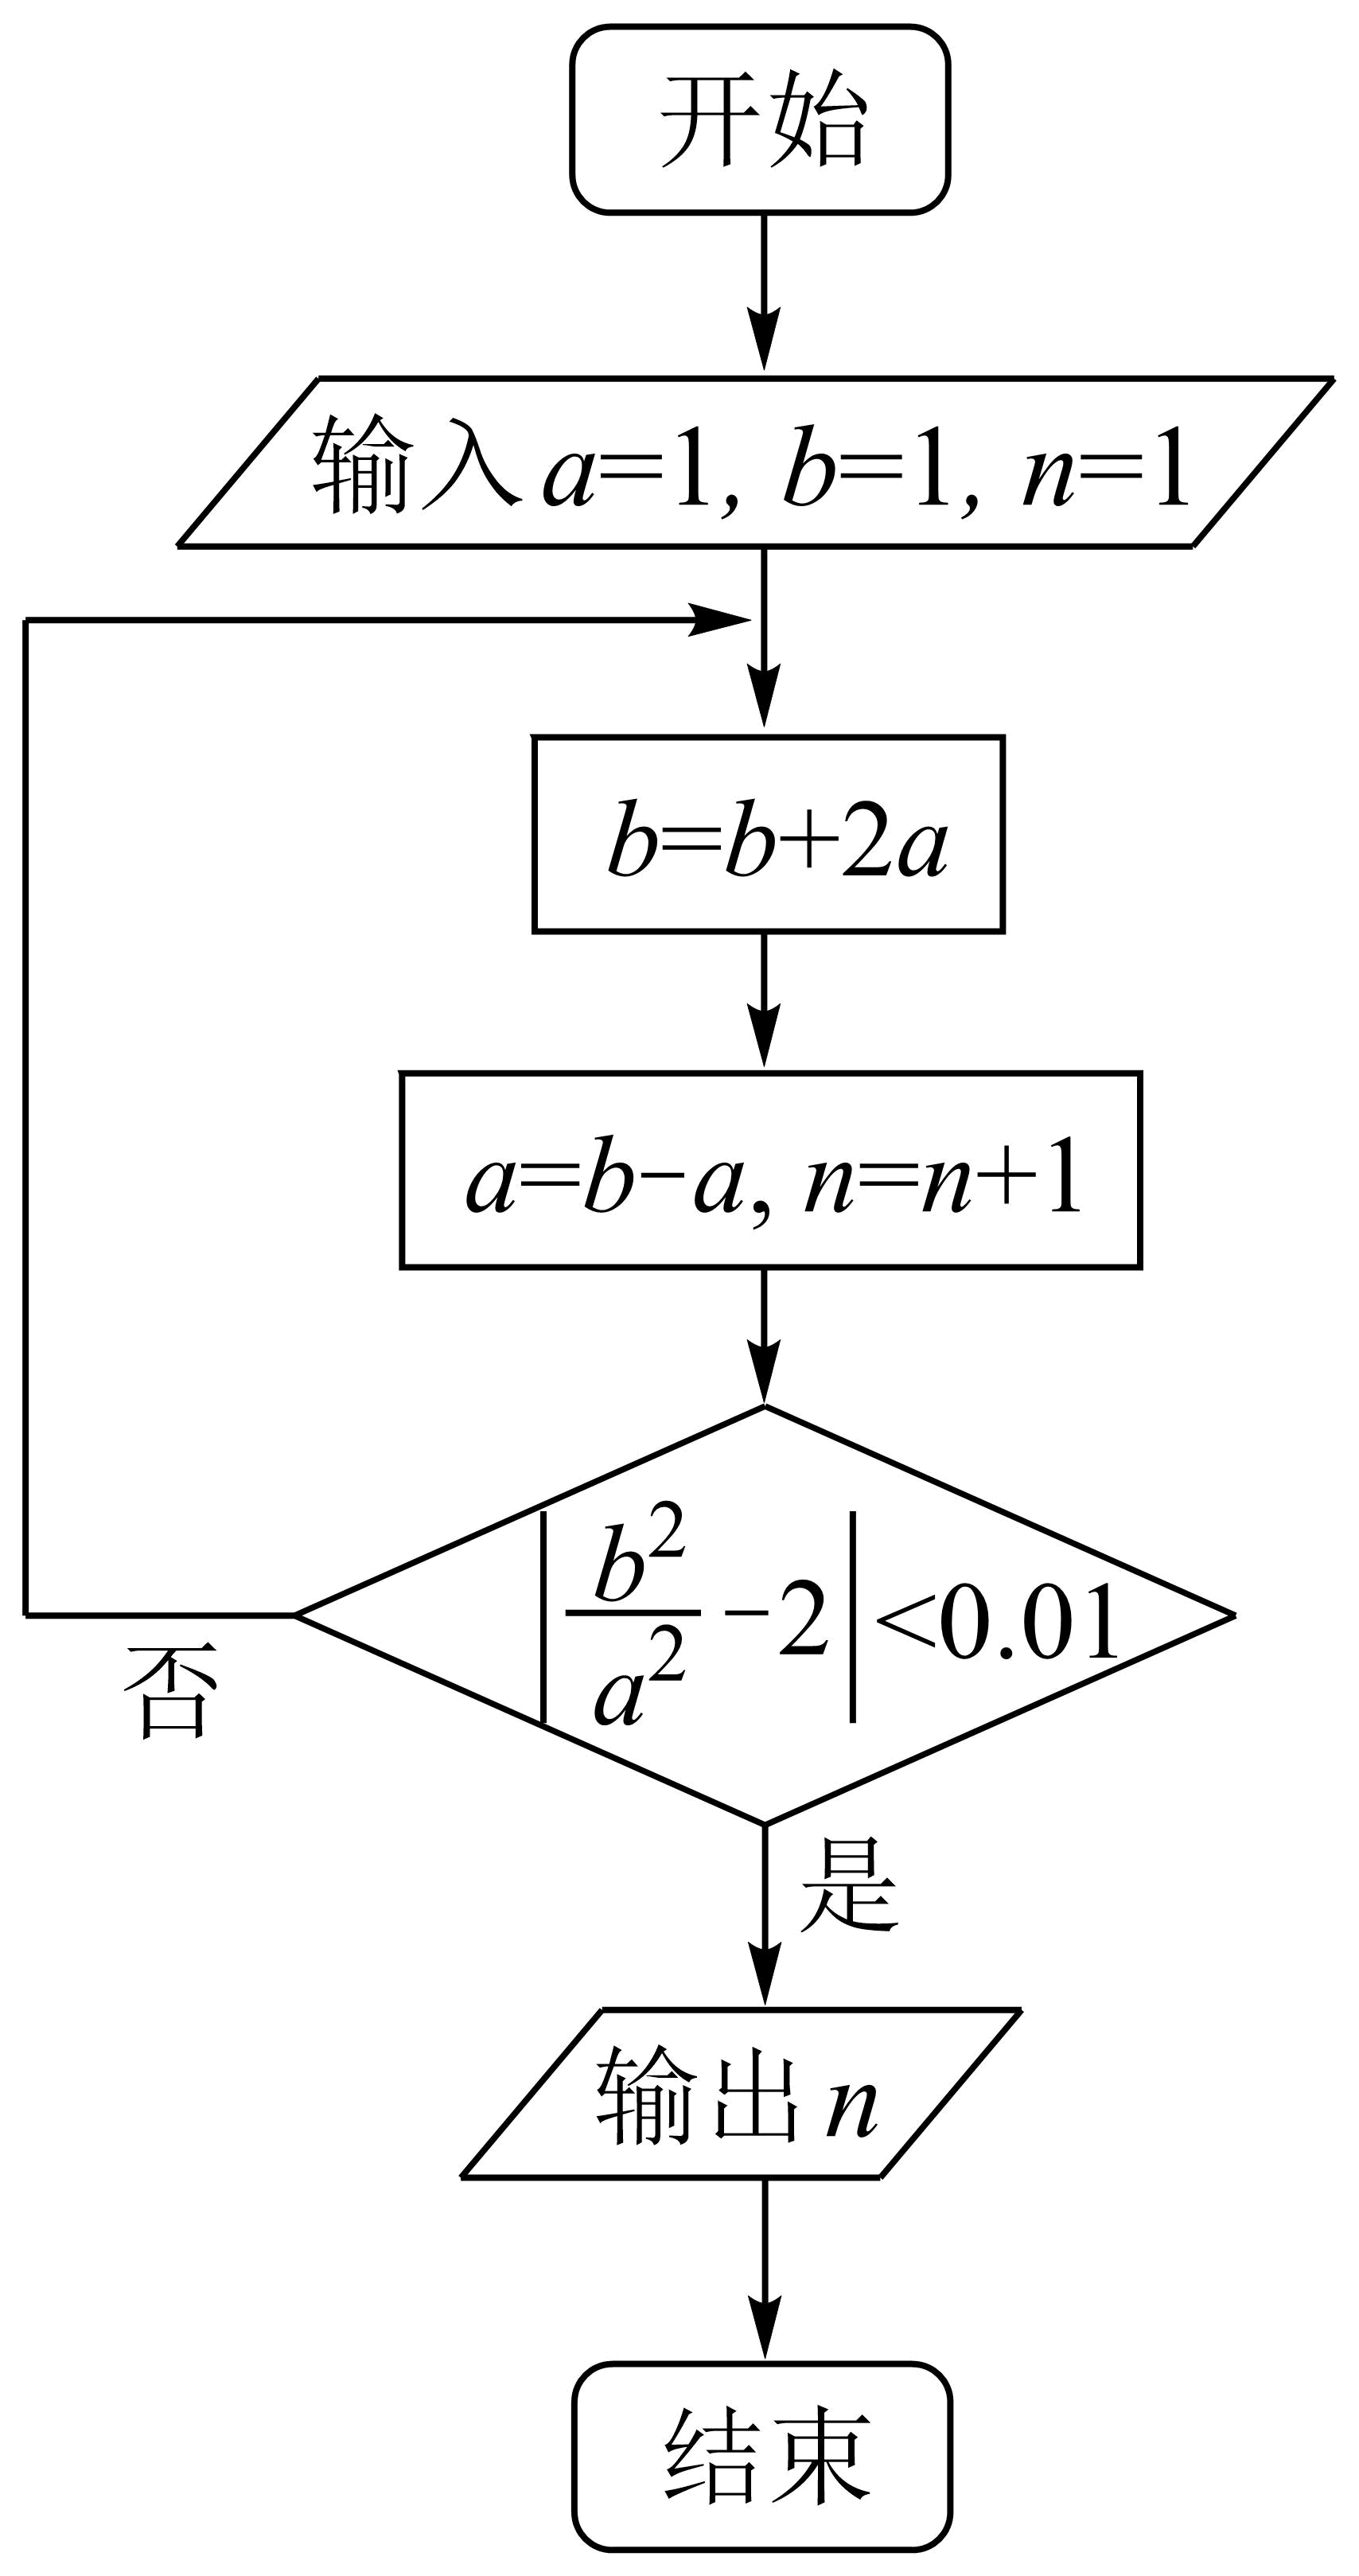
\includegraphics[width=4.6cm]{figures/2022_yili_q6.png}\end{tightcenter}
\fourchoices{$3$}{$4$}{$5$}{$6$}
\item 在正方体 $ABCD-A_1B_1C_1D_1$ 中，$E,F$ 分别为 $AB,BC$ 的中点，则
\twochoices{平面 $B_1EF\perp$ 平面 $BDD_1$}{平面 $B_1EF\perp$ 平面 $A_1BD$}{平面 $B_1EF\parallel$ 平面 $A_1AC$}{平面 $B_1EF\parallel$ 平面 $A_1C_1D$}
\item 已知等比数列 $\{a_n\}$ 的前3项和为168，$a_2-a_5=42$，则 $a_6=$
\fourchoices{$14$}{$12$}{$6$}{$3$}
\item 已知球 $O$ 的半径为1，四棱锥的顶点为 $O$，底面的四个顶点均在球 $O$ 的球面上，则当该四棱锥的体积最大时，其高为
\fourchoices{\tallchoice{$\dfrac13$}}{\tallchoice{$\dfrac12$}}{\tallchoice{$\dfrac{\sqrt3}{3}$}}{\tallchoice{$\dfrac{\sqrt2}{2}$}}
\item 某棋手与甲、乙、丙三位棋手各比赛一盘，各盘比赛结果相互独立. 已知该棋手与甲、乙、丙比赛获胜的概率分别为 $p_1,p_2,p_3$，且 $p_3>p_2>p_1>0$. 记该棋手连胜两盘的概率为 $p$，则
\onechoices{$p$ 与该棋手和甲、乙、丙的比赛次序无关}{该棋手在第二盘与甲比赛，$p$ 最大}{该棋手在第二盘与乙比赛，$p$ 最大}{该棋手在第二盘与丙比赛，$p$ 最大}
\newpage
\item 双曲线 $C$ 的两个焦点为 $F_1,F_2$，以 $C$ 的实轴为直径的圆记为 $D$，过 $F_1$ 作 $D$ 的切线与 $C$ 交于 $M,N$ 两点，且 $\cos\angle F_1NF_2=\dfrac35$，则 $C$ 的离心率为
\fourchoices{\tallchoice{$\dfrac{\sqrt5}{2}$}}{\tallchoice{$\dfrac32$}}{\tallchoice{$\dfrac{\sqrt{13}}2$}}{\tallchoice{$\dfrac{\sqrt{17}}2$}}
\item 已知函数 $f(x),g(x)$ 的定义域均为 $\mathbb R$，且 $f(x)+g(2-x)=5$，$g(x)-f(x-4)=7$. 若 $y=g(x)$ 的图像关于直线 $x=2$ 对称，$g(2)=4$，则 $\sum_{k=1}^{22}f(k)=$
\fourchoices{$-21$}{$-22$}{$-23$}{$-24$}
\end{examquestions}
\examsection{二、填空题：本题共4小题，每小题5分，共20分. }
\begin{examquestions}[start=13]
\item 从甲、乙等5名同学中随机选3名参加社区服务工作，则甲、乙都入选的概率为\blank. 
\item 过四点 $(0,0),(4,0),(-1,1),(4,2)$ 中的三点的一个圆的方程为\blank. 
\item 记函数 $f(x)=\cos(\omega x+\varphi)(\omega>0,0<\varphi<\pi)$ 的最小正周期为 $T$，若 $f(T)=\dfrac{\sqrt3}{2}$，$x=\dfrac\pi9$ 为 $f(x)$ 的零点，则 $\omega$ 的最小值为\blank. 
\item 已知 $x=x_1$ 和 $x=x_2$ 分别是函数 $f(x)=2a^x-e^{x^2}(a>0$ 且 $a\neq1)$ 的极小值点和极大值点. 若 $x_1<x_2$，则 $a$ 的取值范围是\blank. 
\end{examquestions}
\examsection{三、解答题：共70分. 解答应写出文字说明、证明过程或演算步骤. 第17题～第21题为必考题，每个试题考生都必须作答. 第22、23题为选考题，考生根据要求作答. }
\examsection{（一）必考题：共60分. }
\begin{examanswers}[start=17]
\item（12分）

记 $\triangle ABC$ 的内角 $A,B,C$ 的对边分别为 $a,b,c$，已知 $\sin C\sin(A-B)=\sin B\sin(C-A)$. 

（1）证明：$2a^2=b^2+c^2$；

（2）若 $a=5,\cos A=\dfrac{25}{31}$，求 $\triangle ABC$ 的周长. 
\newpage
\item（12分）

如图，四面体 $ABCD$ 中，$AD\perp CD$，$AD=CD$，$\angle ADB=\angle BDC$，$E$ 为 $AC$ 的中点. 

\noindent\begin{minipage}[t]{0.62\linewidth}
（1）证明：平面 $BED\perp$ 平面 $ACD$；

（2）设 $AB=BD=2,\angle ACB=60^\circ$，点 $F$ 在 $BD$ 上，当 $\triangle AFC$ 面积最小时，求 $CF$ 与平面 $ABD$ 所成的角的正弦值. 
\end{minipage}\hfill
\begin{minipage}[t]{0.32\linewidth}\vspace{-1.2em}\centering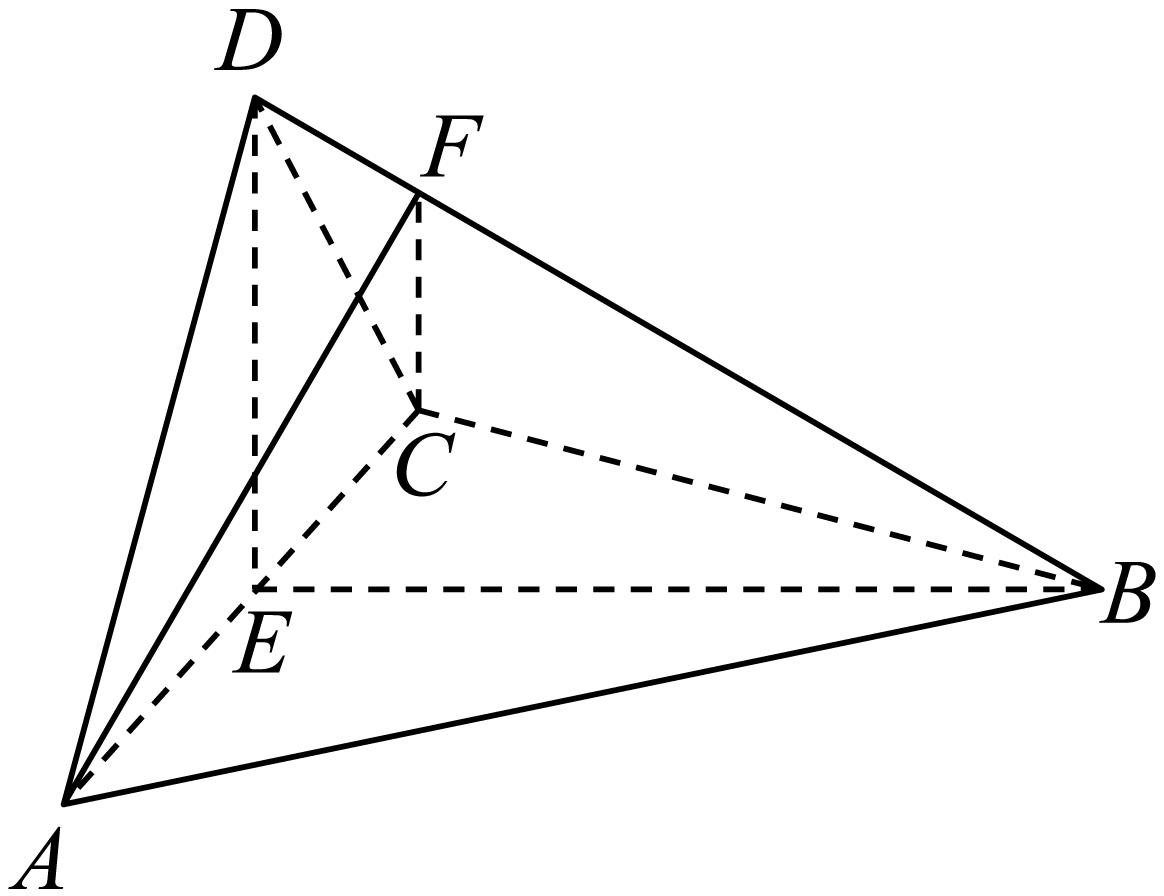
\includegraphics[width=\linewidth]{figures/2022_yili_q18.png}\end{minipage}
\item（12分）

某地经过多年的环境治理，已将荒山改造成了绿水青山. 为估计一林区某种树木的总材积量，随机选取了10棵这种树木，测量每棵树的根部横截面积（单位：$\mathrm{m}^2$）和材积量（单位：$\mathrm{m}^3$），得到如下数据：
\begin{tightcenter}\renewcommand{\arraystretch}{1.35}\begin{tabular}{|c|cccccccccc|c|}\hline 样本号 $i$ & 1&2&3&4&5&6&7&8&9&10&总和\\ \hline 根部横截面积 $x_i$ & 0.04&0.06&0.04&0.08&0.08&0.05&0.05&0.07&0.07&0.06&0.6\\ \hline 材积量 $y_i$ & 0.25&0.40&0.22&0.54&0.51&0.34&0.36&0.46&0.42&0.40&3.9\\ \hline\end{tabular}\end{tightcenter}
并计算得 $\sum_{i=1}^{10}x_i^2=0.038$，$\sum_{i=1}^{10}y_i^2=1.6158$，$\sum_{i=1}^{10}x_iy_i=0.2474$. 

（1）估计该林区这种树木平均一棵的根部横截面积与平均一棵的材积量；

（2）求该林区这种树木的根部横截面积与材积量的样本相关系数（精确到0.01）；

（3）现测量了该林区所有这种树木的根部横截面积，并得到所有这种树木的根部横截面积总和为 $186\mathrm{m}^2$. 已知树木的材积量与其根部横截面积近似成正比. 利用以上数据给出该林区这种树木的总材积量的估计值. 

附：相关系数 $r=\dfrac{\sum_{i=1}^{n}(x_i-\overline x)(y_i-\overline y)}{\sqrt{\sum_{i=1}^{n}(x_i-\overline x)^2\sum_{i=1}^{n}(y_i-\overline y)^2}}$，$\sqrt{1.896}\approx1.377$. 
\item（12分）

已知椭圆 $E$ 的中心为坐标原点，对称轴为 $x$ 轴、$y$ 轴，且过 $A(0,-2),B\left(\dfrac32,-1\right)$ 两点. 

（1）求 $E$ 的方程；

（2）设过点 $P(1,-2)$ 的直线交 $E$ 于 $M,N$ 两点，过 $M$ 且平行于 $x$ 轴的直线与线段 $AB$ 交于点 $T$，点 $H$ 满足 $\overrightarrow{MT}=\overrightarrow{TH}$. 证明：直线 $HN$ 过定点. 
\item（12分）

已知函数 $f(x)=\ln(1+x)+axe^{-x}$. 

（1）当 $a=1$ 时，求曲线 $y=f(x)$ 在点 $(0,f(0))$ 处的切线方程；

（2）若 $f(x)$ 在区间 $(-1,0),(0,+\infty)$ 各恰有一个零点，求 $a$ 的取值范围. 
\end{examanswers}
\examsection{（二）选考题：共10分. 请考生在第22、23题中任选一题作答. 如果多做，则按所做的第一题计分. }
\begin{examanswers}[start=22]
\item（10分）【选修4-4：坐标系与参数方程】

在直角坐标系 $xOy$ 中，曲线 $C$ 的参数方程为\linsys{x=\sqrt3\cos2t,\\ y=2\sin t}（$t$ 为参数），以坐标原点为极点，$x$ 轴正半轴为极轴建立极坐标系，已知直线 $l$ 的极坐标方程为 $\rho\sin\left(\theta+\dfrac\pi3\right)+m=0$. 

（1）写出 $l$ 的直角坐标方程；

（2）若 $l$ 与 $C$ 有公共点，求 $m$ 的取值范围. 
\item（10分）【选修4-5：不等式选讲】

已知 $a,b,c$ 都是正数，且 $a^{\frac32}+b^{\frac32}+c^{\frac32}=1$，证明：

（1）$abc\leq\dfrac19$；

（2）$\dfrac{a}{b+c}+\dfrac{b}{a+c}+\dfrac{c}{a+b}\leq\dfrac1{2\sqrt{abc}}$. 
\end{examanswers}

\end{document}
